\section{Funktionaler Vergleich der Spracherweiterungen}
\label{vergleich}

\subsection{Anforderungen an Spracherweiterungen}
\label{vergleich:anforderungen}

Ein Vergleich der Fähigkeiten der einzelnen Spracherweiterungen erfordert einen
Kriterienkatalog, anhand dessen die Bewertung erfolgen kann. Dabei sind sowohl
die Sicht auf die Daten, also der Umgang der Spracherweiterungen mit den Daten,
als auch die Sicht auf die Aufgaben, also die Transformation der Daten, zu
berücksichtigen.

\subsubsection{Datensicht}
\label{vergleich:anforderungen:datensicht}

Der effiziente Umgang mit großen Datenmengen ist seit jeher eines der
Kernprobleme des \gls{hpc} im Allgemeinen, aber auch heterogener Systeme --
d.h.\ unterschiedlicher Berechnungs-Hardware im selben Rechnersystem -- im
Besonderen. Michael Wong \footnote{Mitglied des C++-Standard-Komitees,
ehemaliger Projektleiter des XL-C++-Compilers der Firma IBM und derzeit
Entwicklungsleiter des Unternehmens Codeplay, das unter anderem den
SYCL-Standard implementiert} bezeichnete in einem Vortrag im November 2018 vor
LLVM-Entwicklern die folgenden Punkte als essentielle Probleme der
Programmierung heterogener Systeme (vgl.~\cite{wong2018}):

\paragraph{Datenbewegung} 
Die Bewegung der Daten ist stets mit Kosten verbunden. Im Allgemeinen ist damit
der Zeitbedarf gemeint, um Daten etwa vom Hauptspeicher des Systems in den
Speicher der GPU zu kopieren. Im weiteren Sinne kann dieser Punkt aber auch
andere Kriterien umfassen, wie z.B.\ den für den Kopiervorgang notwendigen
Energiebedarf, der als Bestandteil des gesamten Energiebedarfs von
\gls{hpc}-Systemen in jüngerer Zeit ebenfalls Gegenstand der Forschung geworden
ist.

Aus der Sicht des Programmierers ist außerdem die Frage relevant, ob die
Datenbewegung \textit{explizit} oder \textit{implizit} erfolgt. Die
\textit{explizite} Datenbewegung hat den Vorteil, dass der Programmierer
jederzeit die volle Kontrolle über die Verschiebung und damit auch über die
Performanz hat, geht jedoch mit einer höheren Programmierkomplexität und damit
Fehleranfälligkeit einher. Überdies wird die volle Kontrolle nicht
notwendigerweise an jeder Stelle gebraucht und bläht damit den Quelltext unnötig
auf. Die Adressräume bleiben bei der expliziten Datenbewegung getrennt (siehe
Abbildung~\ref{vergleich:anforderungen:datensicht:explizitebewegung})

Diesem Ansatz steht die \textit{implizite} Datenbewegung gegenüber. Diese
überlässt den Zeitpunkt und den konkreten Vorgang des Kopierens oder
Verschiebens sowie den Umfang der bewegten Datenmenge der Laufzeitumgebung; aus
Sicht des Programmierers existiert ein virtueller Adressraum, den sich CPU und
GPU teilen (siehe
Abbildung~\ref{vergleich:anforderungen:datensicht:implizitebewegung}).

\begin{figure}[!hbt]
    \centering
    \begin{subfigure}{0.75\textwidth}
        \centering
        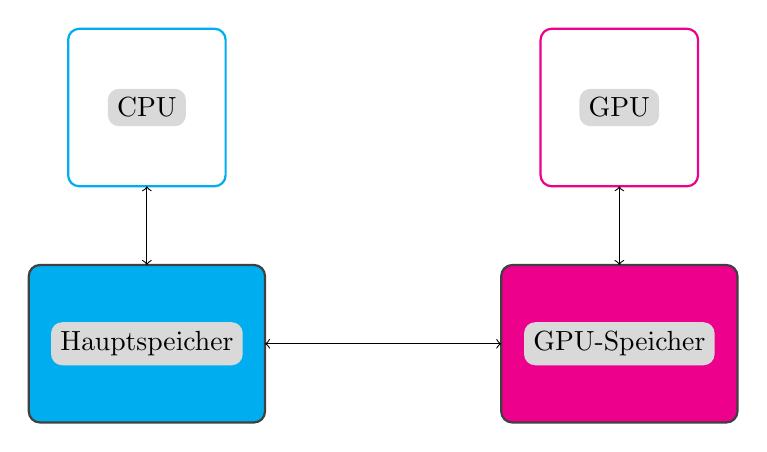
\begin{tikzpicture}
            \draw [thick, rounded corners, draw = cyan]
                  (-1.0, 0.0) rectangle (1.0, 2.0) node[pos = 0.5]
                  {CPU};

            \draw [thick, rounded corners, fill = cyan, draw = darkgray]
                  (-1.5, -3.0) rectangle (1.5, -1.0) node[pos = 0.5]
                  {Hauptspeicher};

            \draw [thick, rounded corners, draw = magenta]
                  (5.0, 0.0) rectangle (7.0, 2.0) node[pos=0.5] {GPU};

            \draw [thick, rounded corners, fill = magenta, draw = darkgray]
                  (4.5, -3.0) rectangle (7.5, -1.0) node[pos = 0.5]
                  {GPU-Speicher};

            \draw [<->] (0.0, 0.0) -- (0.0, -1.0); % CPU <-> RAM
            \draw [<->] (6.0, 0.0) -- (6.0, -1.0); % GPU <-> GPU-RAM
            \draw [<->] (1.5, -2.0) -- (4.5, -2.0); % RAM <-> GPU-RAM
        \end{tikzpicture}
        \caption{Sicht auf den Adressraum bei expliziter Datenbewegung.}
        \label{vergleich:anforderungen:datensicht:explizitebewegung}
    \end{subfigure}
    \par\bigskip
    \begin{subfigure}{0.75\textwidth}
        \centering
        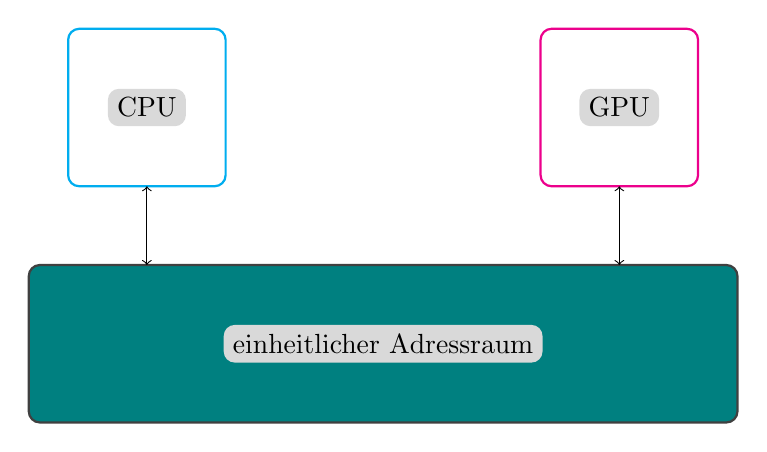
\begin{tikzpicture}
            \draw [thick, rounded corners, draw = cyan]
                  (-1.0, 0.0) rectangle (1.0, 2.0) node[pos = 0.5]
                  {CPU};

            \draw [thick, rounded corners, draw = magenta]
                  (5.0, 0.0) rectangle (7.0, 2.0) node[pos=0.5] {GPU};

            \draw [thick, rounded corners, fill = teal, draw = darkgray]
                  (-1.5, -3.0) rectangle (7.5, -1.0) node[pos = 0.5]
                  {einheitlicher Adressraum};

            \draw [<->] (0.0, 0.0) -- (0.0, -1.0); % CPU <-> Adressraum
            \draw [<->] (6.0, 0.0) -- (6.0, -1.0); % GPU <-> Adressraum
        \end{tikzpicture}
        \caption{Sicht auf den Adressraum bei impliziter Datenbewegung.}
        \label{vergleich:anforderungen:datensicht:implizitebewegung}
    \end{subfigure}
    \caption{Verschiedene Adressraumsichten}
    \label{vergleich:anforderungen:datensicht:adressraeume}
\end{figure}

Eine bewertende Gegenüberstellung beider Ansätze übersteigt den Rahmen dieser
Arbeit. Stattdessen wird untersucht, in welcher Form beide Ansätze von den
jeweiligen Spracherweiterungen unterstützt werden.

\paragraph{Datenanordnung}

Die Anordnung der Daten im Speicher kann aufgrund einer Reihe von Faktoren, wie
etwa unterschiedlicher optimaler Zugriffsmuster von CPUs (\textit{cachelines})
und GPUs (\textit{strided access}), erheblich zur Performanz der Berechnung
beitragen. Aus Sicht des Programmieres ist es daher wünschenswert, dass die
Spracherweiterung eine abstrakte Sicht auf den von ihr verwendeten Speicher
bietet, welche die optimalen Zugriffsmuster der verschiedenen Hardware kapselt.

\paragraph{Datenaffinität}

Die Datenaffinität definiert die Zuordnung und Nähe eines Speicherbereichs zu
einer \textit{bestimmten} Ausführungseinheit, die auf diesen Speicherbereich
zugreifen muss. Im Hinblick auf GPUs meint dies die Zuordnung von im
Hauptspeicher liegenden Daten auf eine oder mehrere GPUs.

\paragraph{Datenlokalität}

Die obigen Punkte sind alle eng mit dem Aspekt der Datenlokalität verknüpft.
Im GPU-Kontext ist vornehmlich relevant, inwiefern sich die einzelnen
Ebenen der Speicherhierarchie (GPU-globaler Speicher, lokaler Speicher und Cache
der auf der GPU verbauten parallelen Prozessoren, Register der einzelnen
Threads) durch die Spracherweiterungen ansteuern und nutzen lassen.

\subsubsection{Aufgabensicht}
\label{vergleich:anforderungen:aufgabensicht}

Die im vorherigen Abschnitt genannten Punkte stellen die in dieser Arbeit
verwendeten Vergleichskriterien dar, bedürfen jedoch noch einer Ergänzung:

\paragraph{Aufgabengraphen}

Viele Anwendungen des \gls{hpc}-Umfelds, wie etwa im Bereich des maschinellen
Lernens oder wissenschaftlicher Berechnungen, haben eine iterative Struktur. Die
Abfolge und Abhängigkeiten einzelner \textit{Kernel} lassen sich in Form eines
Graphen darstellen (siehe
Abbildung~\ref{vergleich:anforderungen:aufgabensicht:graph}). Eine effiziente
Implementierung dieser Graphen setzt voraus, dass Kernel \textit{asynchron} --
sowohl im Hinblick auf die CPU als auch untereinander -- und \textit{parallel}
auf der gleichen GPU ausgeführt werden können. Im Rahmen dieser Arbeit wird
deshalb ebenfalls untersucht, welche Mittel die einzelnen Spracherweiterungen
zur Verfügung stellen, um Aufgabengraphen zu implementieren.

\begin{figure}[htb]
    \centering
    \begin{tikzpicture}
        \tikzstyle{every node} = [node distance = 3cm, fill = gray!30]

        \Vertex{B}
        \NOEA(B){A}
        \SOEA(B){D}
        \NOEA(D){C}

        \tikzstyle{EdgeStyle}=[post]
        \Edge(A)(B)
        \Edge(A)(C)
        \Edge(B)(D)
        \Edge(C)(D)
    \end{tikzpicture}
    \caption{Beispielhafter Aufgabengraph. Der Kernel D hängt von den Kerneln
             B und C ab, die voneinander unabhängig sind, jedoch beide vom
             Kernel A abhängen.}
    \label{vergleich:anforderungen:aufgabensicht:graph}
\end{figure}

\subsection{CUDA}
\label{vergleich:cuda}

\subsubsection{Übersicht}
\label{vergleich:cuda:uebersicht}

Da der CUDA-Compiler \texttt{nvcc} ein C++-Compiler ist, lässt sich CUDA neben
C++ auch in klassischen C-Programmen nutzen, sofern die Inkompatibilitäten
zwischen C und C++ beachtet werden. Zu diesem Zweck ist das \gls{api} auf
C-Konventionen beschränkt und unterstützt C++-Idiome nur sehr begrenzt. Die
CUDA-Kernel selbst werden in einem C++-Dialekt geschrieben.
(vgl.~\cite{cudaguide}, Abschnitt F)

CUDA-Kernel werden gemeinsam mit dem sie aufrufenden Quelltext kompiliert; CUDA
folgt damit dem Modell der \textit{\gls{singlesource}}\footnote{CUDAs frühester
Konkurrent \gls{opencl} kompiliert die Device-Kernel dagegen erst zur Laufzeit
des Programms, um zwischen verschiedenen Architekturen portabel zu bleiben
(\textit{\gls{splitsource}}.)}. \texttt{nvcc} extrahiert dazu die Kernel und
Device-Funktionen aus dem Quelltext und reicht den verbleibenden C- oder
C++-Quelltext an den auf dem System befindlichen entsprechenden Compiler
weiter. Der Device-Quelltext wird in einem weiteren Schritt vom tatsächlichen
Device-Compiler \texttt{cicc} in die Maschinensprache der Ziel-GPU übersetzt.

\subsubsection{Datensicht}
\label{vergleich:cuda:datensicht}

\paragraph{Datenbewegung}

CUDA bietet mehrere Möglichkeiten der Datenbewegung an. Die \textit{explizite}
Datenbewegung wird seit der ersten CUDA-Version unterstützt und erfordert vom
Programmierer die Allokation von Host- und Device-Speicher, das Auslösen des
Kopiervorgangs der Daten vom Host auf das Device (und zurück) und das Freigeben
des Speichers, wenn er nicht mehr benötigt wird (siehe
Quelltext~\ref{vergleich:cuda:datensicht:explizitebewegung}).

\begin{code}
    \begin{minted}[breaklines,breakafter=\,,escapeinside=||,fontsize=\small]{c++}
auto a_h = new float[num_elems];
auto b_h = new float[num_elems];

/* a_h initialisieren */

auto a_d = static_cast<float*>(nullptr);
auto b_d = static_cast<float*>(nullptr);
cudaMalloc(&a_d, num_elems * sizeof(float));
cudaMalloc(&b_d, num_elems * sizeof(float));

cudaMemcpy(a_d, a_h, num_elems * sizeof(float),
           |\textbf{\textcolor{keyword-green}{cudaMemcpyHostToDevice}}|);

kernel<<<...>>>(a_d, b_d, num_elems);

cudaMemcpy(b_h, b_d, num_elems * sizeof(float),
           |\textbf{\textcolor{keyword-green}{cudaMemcpyDeviceToHost}}|);

cudaFree(b_d);
cudaFree(a_d);

delete[] b_h;
delete[] a_h;
    \end{minted}
    \caption{Explizite Datenbewegung mit CUDA}
    \label{vergleich:cuda:datensicht:explizitebewegung}
\end{code}

Seit dem im Jahr 2011 erschienenen CUDA 4 unterstützt CUDA einen einheitlichen
virtuellen Adressraum für Host und Device (vgl.~\cite{cuda2011}, S.\ 4). Dieser
ermöglichte noch keine implizite Datenbewegung, ersparte dem Programmierer
aber die Angabe der Kopierrichtung beim Aufruf von
\mintinline{c++}{cudaMemcpy}. Der letzte Parameter des Befehls konnte seit
diesem Zeitpunkt durch \mintinline{c++}{cudaMemcpyDefault} ersetzt werden.

Die \textit{implizite} Datenbewegung wird seit dem im Jahr 2014 erschienenen
CUDA 6 unterstützt (vgl.~\cite{cuda2014}, S.\ 3). Der Befehl
\mintinline{c++}{cudaMallocManaged} allokiert einen Speicherbereich, der sowohl
vom Host als auch vom Device angesteuert werden kann. Die CUDA-Laufzeitumgebung
sorgt dann im Hintergrund für das Kopieren der notwendigen Speicherbereiche, es
obliegt jedoch dem Programmierer, die Synchronisierung zwischen Host und Device
auszuführen. Das in Quelltext~\ref{vergleich:cuda:datensicht:explizitebewegung}
aufgeführte Beispiel wird dadurch zu der in
Quelltext~\ref{vergleich:cuda:datensicht:implizitebewegung} gezeigten
Vereinfachung.

\begin{code}
    \begin{minted}[breaklines,breakafter=\,,escapeinside=||,fontsize=\small]{c++}
auto a = static_cast<float*>(nullptr);
auto b = static_cast<float*>(nullptr);

cudaMallocManaged(&a, num_elems * sizeof(float));
cudaMallocManaged(&b, num_elems * sizeof(float));

kernel<<<...>>>(a, b, num_elems);

cudaDeviceSynchronize();

/* b ab hier auf dem Host nutzbar */

cudaFree(b);
cudaFree(a);
    \end{minted}
    \caption{Implizite Datenbewegung ab CUDA 6}
    \label{vergleich:cuda:datensicht:implizitebewegung}
\end{code}

Im Jahr 2016 führte NVIDIA die Pascal-Architektur und CUDA 8 ein. Mit dieser
neuen Architektur wurde die implizite Datenbewegung weiter vereinfacht, da es
nun möglich war, gänzlich auf CUDA zur Speicherallokation zu verzichten: der
Aufruf von \mintinline{c++}{new} oder \mintinline{c}{malloc} genügt
(vgl.~\cite{harris2016}). Dadurch wurde auch die Verwendung von C++-Containern
im Zusammenhang mit CUDA einfacher, deren Speicherbereich man nun direkt an
CUDA-Kernel übergeben konnte (siehe
Quelltext~\ref{vergleich:cuda:datensicht:explizitcuda8}).

\begin{code}
    \begin{minted}[breaklines,breakafter=\,,escapeinside=||,fontsize=\small]{c++}
auto a = std::vector<float>{};
auto b = std::vector<float>{};

a.resize(num_elems);
b.resize(num_elems);

kernel<<<...>>>(a.data(), b.data(), num_elems);

cudaDeviceSynchronize();

/* b ab hier auf dem Host nutzbar */
    \end{minted}
    \caption{Implizite Datenbewegung ab CUDA 8 und Pascal}
    \label{vergleich:cuda:datensicht:explizitcuda8}
\end{code}

\paragraph{Datenanordnung}

Die Anordnung der Daten im globalen Speicher der GPU entspricht bei der
Allokation mit \mintinline{c++}{cudaMalloc} und der Kopie mit
\mintinline{c++}{cudaMemcpy} der Anordnung der Daten im Host-Speicher. Es ist
Aufgabe des Programmierers, die Effizienz der Anordnung und des
Zugriffsverhaltens sicherzustellen (vgl.~\cite{cudaguide}, Abschnitt 5.3.2,
Überschrift \glqq Global Memory\grqq).

Einen Sonderfall stellen zweidimensionale Arrays dar. Die Adresse $A$ eines
Felds eines 2D-Arrays mit der Startadresse $S$ und der Breite $B$ durch einen
Thread mit den Koordinaten $(x, y)$ berechnet sich in vielen Anwendungsfällen
wie folgt:

\begin{align*}
    A = S + y * B + x
\end{align*}

Ein effizienter Zugriff dieser Form erfordert sowohl eine Block-Breite als auch
eine Array-Breite, die ein mathematisches Vielfaches der Warpbreite sind. Mit
\mintinline{c++}{cudaMallocPitch} und \mintinline{c++}{cudaMemcpy2D} kann man
letzterer Anforderung Rechnung tragen. Eine Erweiterung dieses Prinzips auf
dreidimensionale Arrays, die man sich auch als Array von 2D-Arrays vorstellen
kann, ist mit \mintinline{c++}{cudaMalloc3D} und \mintinline{c++}{cudaMemcpy3D}
möglich. (vgl.~\cite{cudaguide}, Abschnitt 5.3.2, Überschrift \glqq
Two-Dimensional Arrays\grqq)

Sofern häufig auf benachbarte Spalten und Zeilen eines Arrays zugegriffen
wird, lässt sich dies effizienter auslesen, wenn die eigentlich für
Grafikoperationen -- die häufig benachbarte Pixel manipulieren -- vorgesehenen
Textur-Caches der GPU genutzt werden. Eine für diese Caches optimale
Speicheranordnung lässt sich mit \mintinline{c++}{cudaMallocArray}
bewerkstelligen. Ein auf diese Weise angelegtes \mintinline{c++}{cudaArray} ist
kein Zeiger, sondern eine für den Programmierer opake Datenstruktur, auf die
nur über spezielle Texturbefehle zugegriffen werden kann.
(vgl.~\cite{cudaguide}, Abschnitt 5.3.2, Überschrift \glqq Texture and Surface
Memory\grqq)

\paragraph{Datenaffinität}

\paragraph{Datenlokalität}

\subsubsection{Aufgabensicht}

\paragraph{Aufgabengraphen}

\subsection{HIP}

\subsubsection{Datensicht}

\paragraph{Datenbewegung}

\paragraph{Datenanordnung}

\paragraph{Datenaffinität}

\paragraph{Datenlokalität}

\subsubsection{Aufgabensicht}

\paragraph{Aufgabengraphen}

\subsection{HC}

\subsubsection{Datensicht}

\paragraph{Datenbewegung}

\paragraph{Datenanordnung}

\paragraph{Datenaffinität}

\paragraph{Datenlokalität}

\subsubsection{Aufgabensicht}

\paragraph{Aufgabengraphen}

\subsection{SYCL}

\subsubsection{Datensicht}

\paragraph{Datenbewegung}

\paragraph{Datenanordnung}

\paragraph{Datenaffinität}

\paragraph{Datenlokalität}

\subsubsection{Aufgabensicht}

\paragraph{Aufgabengraphen}

